\item A horizontally flying bullet of mass \(m\) gets stuck in a body of mass \(M\) suspended by two identical threads of length \(l\) (Fig. 1.42).
    \begin{center}
        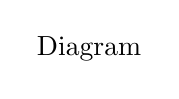
\begin{tikzpicture}
            \node at (0, 0) {Diagram};
        \end{tikzpicture}
    \end{center}
    As a result, the threads swerve through an angle \(\theta\). Assuming \(m \ll M\), find:
    \begin{enumerate}
        \item the velocity of the bullet before striking the body;
        \item the fraction of the bullet's initial kinetic energy that turned into heat.
    \end{enumerate}
\begin{solution}
    \begin{center}
        \begin{tikzpicture}
            \pic at (0, 0) {frame=3cm};
        \end{tikzpicture}
    \end{center}
    
    \begin{align*}
        \intertext{From conservation of momentum, for the system “bullet + body” along the initial direction of bullet}
        m v_0 &= (m + M)v \quad \text{or} \quad v = \dfrac{mv_0}{m + M} \tag{1}
        \intertext{where $v_0$ is the initial velocity of the bullet and $v$ is combined velocity, after the collision.}
    \end{align*}
    
    \begin{align*}
        \intertext{From conservation of mechanical energy of the system (bullet + body) in the field of gravity:}
        \dfrac{1}{2} (m + M) v^2 &= (M + m)g l (1 - \cos \theta) \quad \text{or} \quad v^2 = 2g l (1 - \cos \theta) \tag{2}
        \intertext{(a) From Eqs. (1) and (2),}
        v_0 &= \dfrac{(m + M)}{m} \sqrt{2gl(1 - \cos \theta)} = \dfrac{2(M + m)}{m} \sqrt{gl} \sin (\theta / 2)\\
        \intertext{As $m \ll M$,}
        v_0 &\approx \dfrac{2M}{m} \sqrt{gl} \sin (\theta / 2)
        \intertext{(b) Fraction of initial kinetic energy turned into heat}
        \dfrac{T_i - T_f}{T_i} &= 1 - \dfrac{T_f}{T_i} = 1 - \dfrac{\dfrac{1}{2} (m + M) v^2}{\dfrac{1}{2} mv_0^2}\\
        &= 1 - \dfrac{m}{(m + M)} \approx \left( 1 - \dfrac{m}{M} \right) \quad \text{(using Eq. 1)}
    \end{align*}
\end{solution}
